\documentclass[../main.tex]{subfiles}
\begin{document}

\theoremstyle{definition}

\chapter{Eigenvalues}
\begin{center}
\textbf{CHAPTER OBJECTIVES}
\end{center}
Knowledge and understanding are prerequisites for the effective implementation objectives and topics covered are
\begin{itemize}
\item Understanding the mathematical definition of eigenvalues and eigenvectors.
\item Understanding the physical interpretation of eigenvalues and eigenvectors within
the context of engineering systems that vibrate or oscillate.
\item Knowing how to implement the polynomial method.
\item Knowing how to implement the power method to evaluate the largest and smallest eigenvalues and their respective eigenvectors.
\item Knowing how to use and interpret MATLAB's eig function.
\end{itemize}
\textbf{YOU'VE GOT A PROBLEM }
At the beginning of Chap. 8, we used Newton's second law and force balances to predict the equilibrium positions of three bungee jumpers connected by cords. Because
we assumed that the cords behaved like ideal springs (i.e., followed Hooke's law),
the steady-state solution reduced to solving a system of linear algebraic equations (recall
Eq. 8.1 and Example 8.2). In mechanics, this is referred to as a statics problem.
Now let's look at a dynamics problem involving the same system. That is, we'll study the
jumpers' motion as a function of time. To do this, their initial conditions (i.e., their initial positions and velocities) must be prescribed. For example, we can set the jumpers' initial positions at the equilibrium values computed in Example 8.2. If we then set their initial velocities
to zero, nothing would happen because the system would be at equilibrium.
Because we are now interested in examining the system's dynamics, we must set the
initial conditions to values that induce motion. Although we set the jumpers' initial positions to the equilibrium values and the middle jumper's initial velocity to zero, we set the
upper and bottom jumper's initial velocities to some admittedly extreme values. That is, we

\begin{figure}[H]
		\centering
		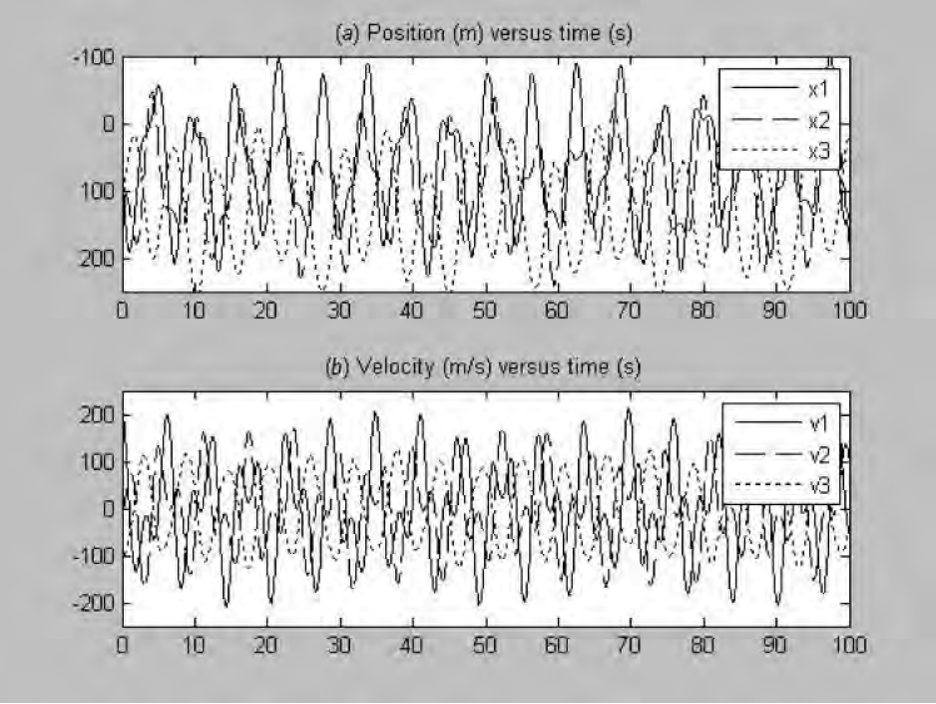
\includegraphics[width=0.75\textwidth]{fig_13_26}
	   \caption{\textsf{The (a) positions and (b) velocities versus time for the system of three interconnected bungee
jumpers from Example 8.2.}}
	   \label{fig:fig_13_26}
\end{figure}

impose a downward velocity of 200 m/s on jumper 1 and an upward velocity of 100 m/s on
jumper 3. (Safety tip: Don't try this at home!) We then used MATLAB to solve the differential
equations (Eq. 8.1) to generate the resulting positions and velocities as a function of time.
\footnote{1 We will show how this is done when we cover ordinary differential equations in Part Six.}


As displayed in Fig. 13.1, the outcome is that the jumpers oscillate wildly. Because
there are no friction forces (e.g., no air drag or spring dampening), they lurch up and down
around their equilibrium positions in a persistent manner that at least visually borders on
the chaotic. Closer inspection of the individual trajectories suggests that there may be some
pattern to the oscillations. For example, the distances between peaks and troughs might be
constant. But when viewed as a time series, it is difficult to perceive whether there is anything systematic and predictable going on.


In this chapter, we deal with one approach for extracting something fundamental out
of such seemingly chaotic behavior. This entails determining the eigenvalues, or characteristic values, for such systems. As we will see, this involves formulating and solving systems of linear algebraic equations in a fashion that differs from what we've done to this
point. To do this, let's first describe exactly what is meant by eigenvalues from a mathematical standpoint.

\section{MATHEMATICAL BACKGROUND}
Chapters 8 through 12 have dealt with methods for solving sets of linear algebraic equations of the general form
\begin{equation}
[A]\{x\}=\{b\} \tag{13.1}
\end{equation}

Such systems are called nonhomogeneous because of the presence of the vector $\{b\}$ on the
right-hand side of the equality. If the equations comprising such a system are linearly
independent (i.e., have a nonzero determinant), they will have a unique solution. In other
words, there is one set of x values that will make the equations balance. As we've already
seen in Sec. 9.1.1, for two equations with two unknowns, the solution can be visualized as
the intersection of two straight lines represented by the equations (recall Fig. 9.1).
In contrast, a homogeneous linear algebraic system has a right-hand side equal to zero:
\begin{equation}
[A]\{x\}=0 \tag{13.2}
\end{equation}

At face value, this equation suggests that the only possible solution would be the trivial
case for which all $x's = 0$. Graphically this would correspond to two straight lines that intersected at zero.
Although this is certainly true, eigenvalue problems associated with engineering are
typically of the general form
\begin{equation}
[[A]-\lambda[I]]\{x\}=0 \tag{13.3}
\end{equation}

where the parameter $\lambda$ is the eigenvalue. Thus, rather than setting the x's to zero, we can
determine the value of $\lambda$ that drives the left-hand side to zero! One way to accomplish this
is based on the fact that, for nontrivial solutions to be possible, the determinant of the matrix must equal zero
\begin{equation}
[[A]-\lambda[I]]=0 \tag{13.4}
\end{equation}

Expanding the determinant yields a polynomial in $\lambda$, which is called the characteristic
polynomial. The roots of this polynomial are the solutions for the eigenvalues.
In order to better understand these concepts, it is useful to examine the two-equation
case,
\begin{equation}
(a_{11}-\lambda)x_{1}+a_{12}x_{2}=0
\end{equation}

\begin{equation}
a_{21}x_{1}+(a_{22}-\lambda)x_{2}=0 \tag{13.5}
\end{equation}

Expanding the determinant of the coefficient matrix gives
\begin{equation}
\begin{vmatrix}
a_{11}-\lambda  &a_{12} \\
a_{12} & a_{11}-\lambda
\end{vmatrix}
=\lambda ^{2}-(a{12}+a_{22})\lambda -a_{12}a_{21} \tag{13.6}
\end{equation}


which is the characteristic polynomial. The quadratic formula can then be used to solve for
the two eigenvalues:
\begin{equation}
\begin{matrix}
\lambda _{1}\\
\lambda _{2}
\end{matrix}
=\frac{(a_{12}-a_{22})^{2}\pm \sqrt{(a_{11}-a_{22})^{2}-4a_{12}a_{21}}}{2} \tag{13.7}
\end{equation}


These are the values that solve Eq. (13.5). Before proceeding, let's convince ourselves that
this approach (which, by the way, is called the polynomial method) is correct.


\section*{EXAMPLE 13.1 The Polynomial Method}

Problem Statement. Use the polynomial method to solve for the eigenvalues of the following homogeneous system:
\begin{equation}
(10-\lambda )x_{1}-5x_{2}=0
\end{equation}

\begin{equation}
-5x_{1}+(10-\lambda )x_{2}=0
\end{equation}

Solution. Before determining the correct solution, let's first investigate the case where
we have an incorrect eigenvalue. For example, if $\lambda = 3$, the equations become
\begin{equation}
7x_{1}-5x_{2}=0
\end{equation}

\begin{equation}
-5x_{1}+7x_{2}=0
\end{equation}

Plotting these equations yields two straight lines that intersect at the origin (Fig. 13.2a).
Thus, the only solution is the trivial case where $x_{1} = x_{2} = 0$.
To determine the correct eigenvalues, we can expand the determinant to give the characteristic polynomial:
\begin{equation}
\begin{vmatrix}
10-\lambda  &-5 \\
-5 & 10-\lambda
\end{vmatrix}
=\lambda ^{2}-20\lambda +75
\end{equation}

which can be solved for
\begin{equation}
\begin{matrix}
\lambda _{1}\\
\lambda _{2}
\end{matrix}
\frac{20\pm \sqrt{20^{2}-4(1)75)}}{2}=15,5
\end{equation}

Therefore, the eigenvalues for this system are 15 and 5.
We can now substitute either of these values back into the system and examine the result. For $\lambda = 15$, we obtain
\begin{equation}
-5x_{1}-5x_{2}=0
\end{equation}

\begin{equation}
-5x_{1}-5x_{2}
\end{equation}

Thus, a correct eigenvalue makes the two equations identical (Fig. 13.2b). In essence as we
move towards a correct eigenvalue the two lines rotate until they lie on top of each other.
Mathematically, this means that there are an infinite number of solutions. But solving
either of the equations yields the interesting result that all the solutions have the property
that $x_{1} = -x_{2}$. Although at first glance this might appear trivial, it's actually quite interesting
as it tells us that the ratio of the unknowns is a constant. This result can be expressed in vector form as
\begin{equation}
\{x\}=\begin{Bmatrix}
-1\\
1
\end{Bmatrix}
\end{equation}

which is referred to as the eigenvector corresponding to the eigenvalue $\lambda = 15$.
In a similar fashion, substituting the second eigenvalue, $\lambda_{2} = 5$, gives

\begin{equation}
5x_{1}-5x_{2}=0
\end{equation}

\begin{equation}
-5x_{1}+5x_{2}=0
\end{equation}

\begin{figure}[H]
		\centering
		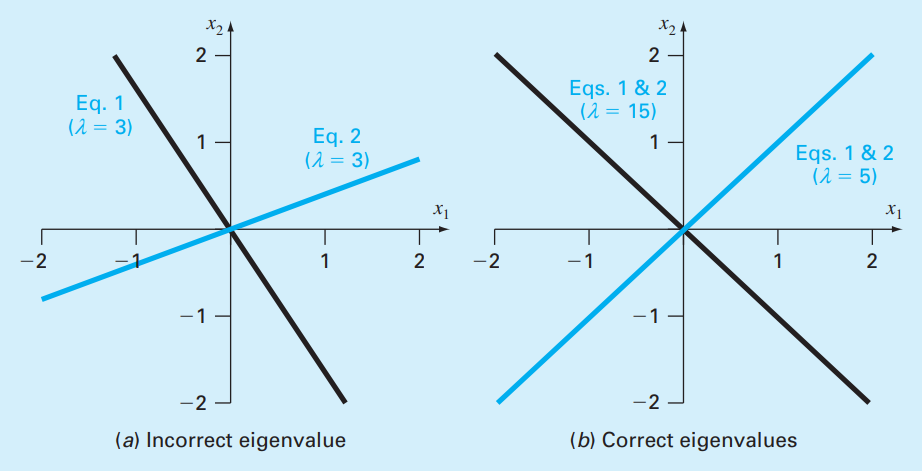
\includegraphics[width=0.75\textwidth]{fig_13_27}
	   \caption{\textsf{Plots of a system of two homogeneous linear equations from Example 13.1. (a) An incorrect
eigenvalue ($\lambda = 3$) means that the two equations, which are labeled as Eq. 1 and 2 in the
figure, plot as separate lines and the only solution is the trivial case ($x_{1} = x_{2} = 0)$. (b) In contrast,
the cases with correct eigenvalues ($\lambda = 5$ and 15), the equations fall on top of each other.}}
	   \label{fig:fig_13_27}
\end{figure}

Again, the eigenvalue makes the two equations identical (Fig. 13.2b) and we can see that
the solution for this case corresponds to $x_{1} = x_{2}$, and the eigenvector is
\begin{equation}
{x}=\begin{Bmatrix}
1\\
1
\end{Bmatrix}
\end{equation}


We should recognize that MATLAB has built-in functions to facilitate the polynomial
method. For Example 13.1, the poly function can be used to generate the characteristic
polynomial as in

\begin{lstlisting}[numbers=none]
>> A = [10 -5;-5 10];
>> p = poly(A)
p =
  1 -20 75
\end{lstlisting}

Then, the roots function can be employed to compute the eigenvalues:
\begin{lstlisting}[numbers=none]
>> d = roots(p)
d =
   15
    5
\end{lstlisting}


The previous example yields the useful mathematical insight that the solution of n
homogeneous equations of the form of Eq. 13.3 consists of a set of n eigenvalues and their
associated eigenvectors. Further, it showed that the eigenvectors provide the ratios of the
unknowns representing the solution. In the next section, we will show how such information has utility in engineering and
science by turning back to our physical problem setting of oscillating objects. However,
before doing so, we'd like to make two more mathematical points.
First, inspection of Fig. 13.2b indicates that the straight lines representing each eigenvalue solution are at right angles to each other. That is, they are orthogonal. This property
is true for symmetric matrices with distinct eigenvalues.
Second, multiplying out Eq. 13.3 and separating terms gives
\begin{equation}
[A]\{x\}=\lambda\{x\}
\end{equation}

When viewed in this way, we can see that solving for the eigenvalues and eigenvectors
amounts to translating the information content of a matrix [A] into a scalar $\lambda$. This might
not seem significant for the 2 × 2 system we have been examining, but it is pretty remarkable when we consider that the size of [A] can potentially be much larger.


\section*{13.2 PHYSICAL BACKGROUND}
The mass-spring system in Fig. 13.3a is a simple context to illustrate how eigenvalues occur
in physical problem settings. It will also help to demonstrate some of the mathematical
concepts introduced in the previous section.
To simplify the analysis, assume that each mass has no external or damping forces
acting on it. In addition, assume that each spring has the same natural length l and the same
spring constant k. Finally, assume that the displacement of each spring is measured relative
to its own local coordinate system with an origin at the spring's equilibrium position
(Fig. 13.3a). Under these assumptions, Newton's second law can be employed to develop
a force balance for each mass:
\begin{equation}
m_{1}\frac{d^{2}x_{1}}{dt^{2}}=-kx_{1}+k(x_{2}-x_{1})\tag{13.8a}
\end{equation}


\begin{figure}[H]
		\centering
		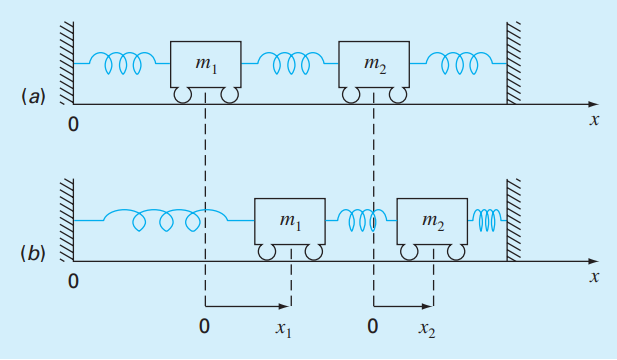
\includegraphics[width=0.75\textwidth]{fig_13_28}
	   \caption{\textsf{Plots of a system of two homogeneous linear equations from Example 13.1. (a) An incorrect
eigenvalue ( two mass–three spring system with frictionless rollers vibrating between two fixed walls.
The position of the masses can be referenced to local coordinates with origins at their respective
equilibrium positions (a). As in (b), positioning the masses away from equilibrium creates forces
in the springs that on release lead to oscillations of the masses.), the equations fall on top of each other.}}
	   \label{fig:fig_13_28}
\end{figure}


\begin{equation}
m_{1}\frac{d^{2}x_{1}}{dt^{2}}=k(x_{2}-x_{1})-kx_{1}\tag{13.8b}
\end{equation}


	where $x_{i}$ is the displacement of mass i away from its equilibrium position (Fig. 13.3b).
From vibration theory, it is known that solutions to Eq. (13.8) can take the form
\begin{equation}
x_{1}=X_{i}sin(\omega t)\tag{13.9}
\end{equation}

where $X_{1} =$ the amplitude of the oscillation of mass i (m) and $\omega =$ the angular frequency
of the oscillation (radians/time), which is equal to

\begin{equation}
\omega =\frac{2\pi }{T_{p}}\tag{13.10}
\end{equation}


where $T_{p}$ = the period (time/cycle). Note that the inverse of the period is called the ordinary frequency f (cycles/time). If time is measured in seconds, the unit for f is the cycles/s,
which is referred to as a Hertz (Hz).
Equation (13.9) can be differentiated twice and substituted into Eq. (13.8). After collection of terms, the result i
\begin{equation}
\left ( \frac{2k}{m_{1}}-\omega ^{2}\right )x_{1}-\frac{k}{m_{1}}x_{2}=0\tag{13.11a}
\end{equation}


\begin{equation}
-\frac{k}{m_{1}}x_{1}+\left ( \frac{2k}{m_{2}}-\omega ^{2} \right )x_{2}=0 \tag{13.11b}
\end{equation}


Comparison of Eq. (13.11) with Eq. (13.3) indicates that at this point, the solution has
been reduced to an eigenvalue problem—where, for this case, the eigenvalue is the square
of the frequency. For a two-degree-of-freedom system such as Fig. 13.3, there will be two
such values along with their eigenvectors. As shown in the following example, the latter
establish the unique relationship between the unknowns.

\section*{EXAMPLE 13.2 Physical Interpretation of Eigenvalues and Eigenvectors}
Problem Statement. If $m_{1} = m_{2} = 40$ kg and k = 200 N/m, Eq. (13.11) is
\begin{equation}
(10-\lambda )x_{1}-5x_{2}=0
\end{equation}

\begin{equation}
-5x_{2}+(10-\lambda )x_{1}=0
\end{equation}

Mathematically, this is the same system we already solved with the polynomial methods in
Example 13.2. Thus, the two eigenvalues are $\omega_{2} = 15$ and 5 s-2 and the corresponding
eigenvectors are $X_{1} = X_{2}$ and $X_{1} = -X_{2}$. Interpret these results as they relate to the massspring system of Fig. 13.3.


Solution. This example provides valuable information regarding the behavior of the system in Fig. 13.3. First, it tells us that the system has two primary modes of oscillation with
angular frequencies of $\omega = 3.873$ and 2.36 radians $s^{-1}$, respectively. These values can be
also expressed as periods (1.62 and 2.81 s, respectively) or ordinary frequencies (0.6164 and 0.3559 Hz, respectively).
As stated in Section 13.1, a unique set of values cannot be obtained for the unknown
amplitudes X. However, their ratios are specified by the eigenvectors. Thus, if the system
\begin{figure}[H]
		\centering
		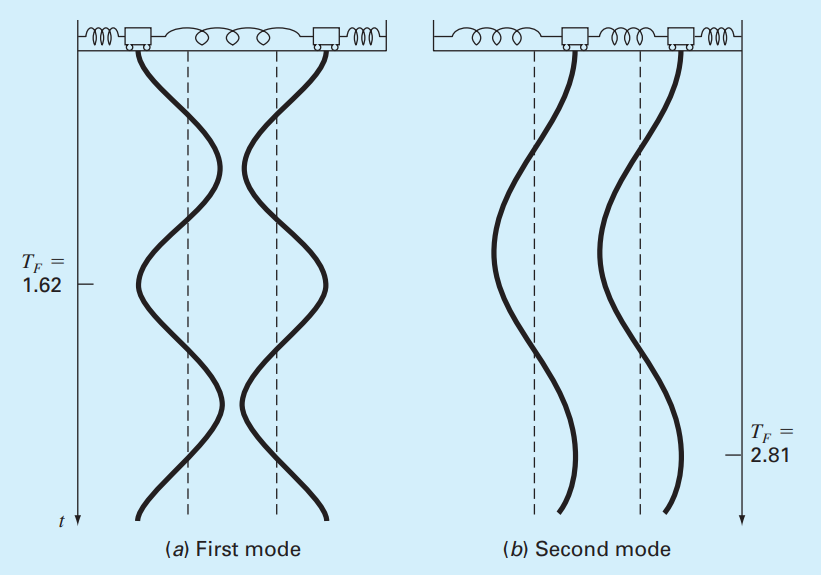
\includegraphics[width=0.75\textwidth]{fig_13_29}
	   \caption{\textsf{The principal modes of vibration of two equal masses connected by three identical springs
between fixed walls.}}
	   \label{fig:fig_13_29}
\end{figure}
is vibrating in the first mode, the first eigenvector tells us that the amplitude of the second
mass will be equal but of opposite sign to the amplitude of the first. As in Fig. 13.4a, the
masses vibrate apart and then together indefinitely (like two hands clapping every 1.62 s).
In the second mode, the eigenvector specifies that the two masses have equal
amplitudes at all times. Thus, as in Fig. 13.4b, they vibrate back and forth in unison every
2.81 s. We should note that the configuration of the amplitudes provides guidance on how
to set their initial values to attain pure motion in either of the two modes. Any other configuration will lead to superposition of the modes. It is this superposition that leads to the
apparently chaotic behavior of systems like the bungee jumpers in Fig. 13.1. But as this example should make clear, there is an underlying systematic behavior that is embodied by
the eigenvalues.


\section*{13.3 THE POWER METHOD}
The power method is an iterative approach that can be employed to determine the largest
or dominant eigenvalue. With slight modification, it can also be employed to determine the
smallest value. It has the additional benefit that the corresponding eigenvector is obtained
as a by-product of the method. To implement the power method, the system being analyzed
is expressed in the form
\begin{equation}
[A]\{x\}=\lambda\{x\}\tag{13.12}
\end{equation}

As illustrated by the following example, Eq. (13.12) forms the basis for an iterative
solution technique that eventually yields the highest eigenvalue and its associated
eigenvector.


\section*{EXAMPLE 13.3 Power Method for Highest Eigenvalue}
Problem Statement. Using the same approach as in Section 13.2, we can derive the following homogeneous set of equations for a three mass–four spring system between two
fixed walls:
\begin{equation}
\left ( \frac{2k}{m_{1}}-\omega^{2}  \right )X_{1}    -\frac{k}{m_{1}}X_{2}=0
\end{equation}


\begin{equation}
-\frac{k}{m_{2}}X_{1}+\left ( \frac{2k}{m_{2}}-\omega ^{2} \right )X_{2}-\frac{k}{m_{2}}X_{3}=0
\end{equation}
\begin{equation}
-\frac{k}{m_{3}}X_{2}+\left ( \frac{k}{m_{2}}-\omega^{2} \right )X_{3}=0
\end{equation}
If all the masses m = 1 kg and all the spring constants k = 20 N/m, the system can be
expressed in the matrix format of Eq. (13.4) as
\begin{equation}
\begin{bmatrix}
40 & -20 & 0\\
-20 & 40 & -20\\
0 & -20 & 40
\end{bmatrix}
-\lambda [I]=0
\end{equation}


where the eigenvalue $\lambda$ is the square of the angular frequency $\omega^{2}$. Employ the power
method to determine the highest eigenvalue and its associated eigenvector.

Solution. The system is first written in the form of Eq. (13.12):
\begin{equation}
40X_{1}-20X_{2}=\lambda X_{1}
\end{equation}

\begin{equation}
-20X_{1}+40X_{2}-20X_{3}=\lambda X_{2}
\end{equation}

\begin{equation}
-20X_{2}+40X_{3}=\lambda X_{3}
\end{equation}

At this point, we can specify initial values of the X's and use the left-hand side to compute
an eigenvalue and eigenvector. A good first choice is to assume that all the X's on the lefthand side of the equation are equal to one
\begin{equation}
40(1) - 20(1) = 20
\end{equation}

\begin{equation}
-20(1) + 40(1) - 20(1) = 0
\end{equation}

\begin{equation}
- 20(1) + 40(1) = 20
\end{equation}

Next, the right-hand side is normalized by 20 to make the largest element equal to one:
\begin{equation}
\begin{Bmatrix}
20\\
0\\
20
\end{Bmatrix}
= 20\begin{Bmatrix}
1\\
0\\
1
\end{Bmatrix}
\end{equation}

Thus, the normalization factor is our first estimate of the eigenvalue (20) and the corresponding eigenvector is $\{1 0 1\}^{T}$
. This iteration can be expressed concisely in matrix form as
\begin{equation}
\begin{bmatrix}
40 & -20 &0 \\
-20 & 40 & -20\\
0 & -20 & 40
\end{bmatrix}
\begin{Bmatrix}
1\\
1\\
1
\end{Bmatrix}
=\begin{Bmatrix}
20\\
0\\
20
\end{Bmatrix}
=20\begin{Bmatrix}
1\\
0\\
1
\end{Bmatrix}
\end{equation}

 next iteration consists of multiplying the matrix by the eigenvector from the last iteration, $\{1 0 1\}^{T}$ to give

 \begin{equation}
 \begin{bmatrix}
40 & -20 &0 \\
-20 & 40 & -20\\
0 & -20 & 40
\end{bmatrix}
\begin{Bmatrix}
1\\
0\\
1
\end{Bmatrix}
=\begin{Bmatrix}
40\\
-40\\
40
\end{Bmatrix}=
40\begin{Bmatrix}
1\\
-1\\
1
\end{Bmatrix}
 \end{equation}

Therefore, the eigenvalue estimate for the second iteration is 40, which can be employed to
determine an error estimate:

\begin{equation}
\begin{vmatrix}
\varepsilon _{a}
\end{vmatrix}
=\begin{vmatrix}
\frac{40-20}{40}
\end{vmatrix}\times 100\%=50\%
\end{equation}

The process can then be repeated.
Third iteration:

\begin{equation}
\begin{bmatrix}
40 & -20 &0 \\
-20 & 40 & -20\\
0 & -20 & 40
\end{bmatrix}\begin{Bmatrix}
1\\
-1\\
1
\end{Bmatrix}=\begin{Bmatrix}
60\\
-80\\
60
\end{Bmatrix}=-80\begin{Bmatrix}
-0.75\\
1\\
-0.75
\end{Bmatrix}
\end{equation}

where $\begin{vmatrix}
\varepsilon _{a}
\end{vmatrix}=150\%$  (which is high because of the sign change).
Fourth iteration:

\begin{equation}
\begin{bmatrix}
40 & -20 &0 \\
-20 & 40 & -20\\
 0& -20 & 40
\end{bmatrix}
\begin{Bmatrix}
-0.75\\
1\\
-0.75
\end{Bmatrix}=\begin{Bmatrix}
-50\\
70\\
-50
\end{Bmatrix}=70\begin{Bmatrix}
-0.71429\\
1\\
-0.71429
\end{Bmatrix}
\end{equation}

where $\begin{vmatrix}
\varepsilon _{a}
\end{vmatrix}=214\%$  (another sign change).
Fifth iteration:

\begin{equation}
\begin{bmatrix}
40 & -20 & 0\\
-20 & 40 & -20\\
0 & -20 & 40
\end{bmatrix}\begin{Bmatrix}
-0.71429\\
1\\
-0.71429
\end{Bmatrix}=\begin{Bmatrix}
-48.51714\\
68.51714\\
-48.51714
\end{Bmatrix}=68.51714\begin{Bmatrix}
-0.70833\\
1\\
-0.70833
\end{Bmatrix}
\end{equation}

where $\begin{vmatrix}
\varepsilon _{a}
\end{vmatrix}=2.08\%$

Thus, the eigenvalue is converging. After several more iterations, it stabilizes on a
value of 68.28427 with a corresponding eigenvector of $\{-0.707107 1 -0.707107\}_{T}$.


Note that there are some instances where the power method will converge to the secondlargest eigenvalue instead of to the largest. James, Smith, and Wolford (1985) provide an
illustration of such a case. Other special cases are discussed in Fadeev and Fadeeva (1963).
In addition, there are sometimes cases where we are interested in determining the
smallest eigenvalue. This can be done by applying the power method to the matrix inverse
of [A]. For this case, the power method will converge on the largest value of $1/\lambda$ - in other words, the smallest value of $\lambda$. An application to find the smallest eigenvalue will be left as
a problem exercise.
Finally, after finding the largest eigenvalue, it is possible to determine the next highest
by replacing the original matrix by one that includes only the remaining eigenvalues. The
process of removing the largest known eigenvalue is called deflation.
We should mention that although the power method can be used to locate intermediate
values, better methods are available for cases where we need to determine all the eigenvalues as described in the next section. Thus, the power method is primarily used when we
want to locate the largest or the smallest eigenvalue.


\section*{13.4 MATLAB FUNCTION: eig}

As might be expected, MATLAB has powerful and robust capabilities for evaluating eigenvalues and eigenvectors. The function eig, which is used for this purpose, can be employed
to generate a vector of the eigenvalues as in

\begin{lstlisting}[numbers=none]
>>  e = eig(A)
\end{lstlisting}

where e is a vector containing the eigenvalues of a square matrix A. Alternatively, it can be
invoked as

\begin{lstlisting}[numbers=none]
>>  [V,D] = eig(A)
\end{lstlisting}

where D is a diagonal matrix of the eigenvalues and V is a full matrix whose columns are
the corresponding eigenvectors.
It should be noted that MATLAB scales the eigenvectors by dividing them by their
Euclidean distance. Thus, as shown in the following example, although their magnitude
may be different from values computed with say the polynomial method, the ratio of their
elements will be identical.


\section*{EXAMPLE 13.4 Eigenvalues and Eigenvectors with MATLAB}

Problem Statement. Use MATLAB to determine all the eigenvalues and eigenvectors
for the system described in Example 13.3.
Solution. Recall that the matrix to be analyzed is
\begin{equation}
\begin{bmatrix}
40 & -20 & 0\\
-20 & 40 & -20\\
0 & -20 & 40
\end{bmatrix}
\end{equation}

The matrix can be entered as
\begin{lstlisting}[numbers=none]
>> A = [40 -20 0;-20 40 -20;0 -20 40];
\end{lstlisting}

If we just desire the eigenvalues, we can enter
\begin{lstlisting}[numbers=none]
>> e = eig(A)
e =
11.7157
40.0000
68.2843
\end{lstlisting}

e that the highest eigenvalue (68.2843) is consistent with the value previously determined with the power method in Example 13.3.

If we want both the eigenvalues and eigenvectors, we can enter
\begin{lstlisting}[numbers=none]
>> [v,d] = eig(A)
v =
0.5000 -0.7071 -0.5000
0.7071 -0.0000 0.7071
0.5000 0.7071 -0.5000
d =
11.7157 0 0
0 40.0000 0
0 0 8.2843
\end{lstlisting}

Although the results are scaled differently, the eigenvector corresponding to the highest eigenvalue $\{-0.5 0.7071 -0.5\}_{T}$ is consistent with the value previously determined
with the power method in Example 13.3: $\{-0.707107 1 -0.707107\}_{T}$
. The can be demonstrated by dividing the eigenvector from the power method by its Euclidean norm:
\begin{lstlisting}[numbers=none]
>> vpower = [-0.7071 1 -0.7071]';
>> vMATLAB = vpower/norm(vpower)
vMATLAB =
-0.5000
0.7071
-0.5000
\end{lstlisting}

Thus, although the magnitudes of the elements differ, their ratios are identical.


\section*{13.5 CASE STUDY EIGENVALUES AND EARTHQUAKES}

Background. Engineers and scientists use mass-spring models to gain insight into
the dynamics of structures under the influence of disturbances such as earthquakes. Figure 13.5 shows such a model for a three-story building. Each floor mass is represented by
mi, and each floor stiffness is represented by ki for i = 1 to 3.
\begin{figure}[H]
		\centering
		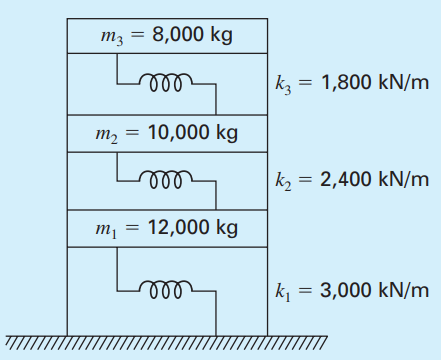
\includegraphics[width=0.75\textwidth]{fig_13_30}
	   \caption{\textsf{A three-story building modeled as a mass-spring system.}}
	   \label{fig:fig_13_30}
\end{figure}

For this case, the analysis is limited to horizontal motion of the structure as it is subjected
to horizontal base motion due to earthquakes. Using the same approach as developed in
Section 13.2, dynamic force balances can be developed for this system as
\begin{equation}
\left ( \frac{k_{1}+k_{2}}{m_{1}}-\omega ^{2}_{n} \right )X_{1} - \frac{k_{2}}{m_{1}}X_{2}=0
\end{equation}

\begin{equation}
-\frac{k_{2}}{m_{2}}X_{1}+\left ( \frac{k_{2}+k_{3}}{m_{2}}-\omega ^{2}_{n} \right )X_{2}-\frac{k_{3}}{m_{2}}X_{3}=0
\end{equation}

\begin{equation}
-\frac{k_{3}}{m_{3}}X_{2}+\left ( \frac{k_{3}}{m_{3}}-\omega ^{2}_{n} \right )X_{3}=0
\end{equation}

where $X_{i}$ represent horizontal floor translations (m), and $\omega_{n}$ is the natural, or resonant, frequency (radians/s). The resonant frequency can be expressed in Hertz (cycles/s) by dividing it by $2\pi$ radians/cycle.
Use MATLAB to determine the eigenvalues and eigenvectors for this system. Graphically represent the modes of vibration for the structure by displaying the amplitudes versus height for each of the eigenvectors. Normalize the amplitudes so that the translation of
the third floor is one.

Solution. The parameters can be substituted into the force balances to give
\begin{equation}
\left ( 450-\omega^{2}_{n} \right )X_{1}-200X_{2}=0
\end{equation}

\begin{equation}
-240X_{1}+\left ( 420-\omega^{2}_{n} \right )X_{2}-180X_{3}=0
\end{equation}

\begin{equation}
-225X_{2}+\left (225-\omega^{2}_{n} \right )X_{3}=0
\end{equation}

A MATLAB session can be conducted to evaluate the eigenvalues and eigenvectors as

\begin{lstlisting}[numbers=none]
>> A=[450 -200 0;-240 420 -180;0 -225 225];
>> [v,d]=eig(A)
v =
-0.5879 -0.6344 0.2913
0.7307 -0.3506 0.5725
-0.3471 0.6890 0.7664
d =
698.5982 0 0
0 339.4779 0
0 0 56.9239
\end{lstlisting}

Therefore, the eigenvalues are 698.6, 339.5, and 56.92 and the resonant frequencies in
Hz are
\begin{lstlisting}[numbers=none]
>> wn=sqrt(diag(d))'/2/pi
wn =
4.2066 2.9324 1.2008
\end{lstlisting}

\begin{figure}[H]
		\centering
		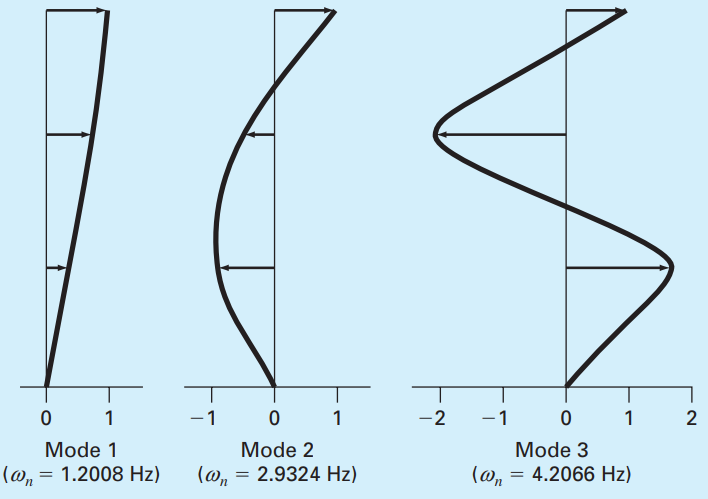
\includegraphics[width=0.75\textwidth]{fig_13_31}
	   \caption{\textsf{The three primary modes of oscillation of the three-story building}}
	   \label{fig:fig_13_31}
\end{figure}

The corresponding eigenvectors are (normalizing so that the amplitude for the third floor is one)
\begin{equation}
\begin{Bmatrix}
1.6934\\
-2.1049\\
1
\end{Bmatrix}
\begin{Bmatrix}
-0.9207\\
-0.5088\\
1
\end{Bmatrix}
\begin{Bmatrix}
0.3801\\
0.7470\\
1 \end{Bmatrix}
\end{equation}

A graph can be made showing the three modes (Fig. 13.6). Note that we have ordered
them from the lowest to the highest natural frequency as is customary in structural
engineering.
Natural frequencies and mode shapes are characteristics of structures in terms of their
tendencies to resonate at these frequencies. The frequency content of an earthquake
typically has the most energy between 0 to 20 Hz and is influenced by the earthquake magnitude, the epicentral distance, and other factors. Rather than a single frequency, they
contain a spectrum of all frequencies with varying amplitudes. Buildings are more receptive
to vibration at their lower modes of vibrations due to their simpler deformed shapes and
requiring less strain energy to deform in the lower modes. When these amplitudes coincide
with the natural frequencies of buildings, large dynamic responses are induced, creating
large stresses and strains in the structure's beams, columns, and foundations. Based on
analyses like the one in this case study, structural engineers can more wisely design buildings to withstand earthquakes with a good factor of safety


STRONA 337
\section{PROBLEMS}
13.1 Repeat Example 13.1 but for three masses with the m's =
40 kg and the k's = 240 N/m. Produce a plot like Fig. 13.4 to
identify the principle modes of vibration.
13.2 Use the power method to determine the highest eigenvalue and corresponding eigenvector for
\begin{equation}
\begin{bmatrix}
2-\lambda  & 8 &10 \\
8 & 4-\lambda & 5\\
10 & 5 & 7-\lambda
\end{bmatrix}
\end{equation}

13.3 Use the power method to determine the lowest eigenvalue and corresponding eigenvector for the system from
Prob. 13.2.
13.4 Derive the set of differential equations for a three
mass–four spring system (Fig. P13.4) that describes their time
motion. Write the three differential equations in matrix form
{Acceleration vector} + [k/m matrix]
{displacement vector x} = 0
Note each equation has been divided by the mass. Solve for
the eigenvalues and natural frequencies for the following
values of mass and spring constants: $k_{1} = k_{4} = 15$ N/m,
$k_{2} = k_{3} = 35$ N/m, and $m_{1} = m_{2} = m_{3} = 1.5$ kg.
3.5 Consider the mass-spring system in Fig. P13.5. The frequencies for the mass vibrations can be determined by solving
for the eigenvalues and by applying $M\ddot{x} + kx = 0$, which
yields
\begin{equation}
\begin{bmatrix}
m_{1} & 0 &0 \\
 0& m_{2} & 0\\
 0&0  & m_{3}
\end{bmatrix}\begin{Bmatrix}
\ddot{x}_{1}\\
\ddot{x}_{2}\\
\ddot{x}_{3}
\end{Bmatrix}+\begin{Bmatrix}
2k & -k & -k\\
-k & 2k & -k\\
 -k& -k & 2k
\end{Bmatrix}\begin{Bmatrix}
x_{1}\\
x_{2}\\
x_{3}
\end{Bmatrix}=\begin{Bmatrix}
0\\
0\\
0
\end{Bmatrix}
\end{equation}

pplying the guess $x = x_{0}e^{i \omega t}$ as a solution, we get the following matrix:
\begin{equation}
\begin{bmatrix}
2k-m_{1}\omega^{2} &-k  & -k\\
 -k& 2k-m_{2}\omega^{2} & -k\\
-k & -k & 2k-m_{3}\omega^{2}
\end{bmatrix}\begin{Bmatrix}
x_{01}\\
x_{02}\\
x_{03}
\end{Bmatrix}e^{i \omega t}=\begin{Bmatrix}
0\\
0\\
0
\end{Bmatrix}
\end{equation}

\begin{figure}[H]
		\centering	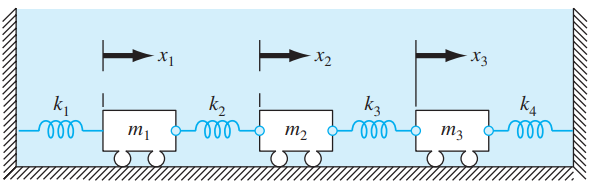
\includegraphics[width=0.75\textwidth]{fig_13_34}
	   \label{fig:fig_13_34}
\end{figure}

\begin{figure}[H]
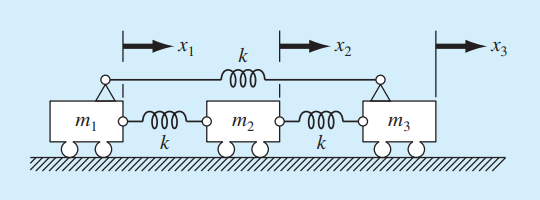
\includegraphics[width=0.75\textwidth]{fig_13_32}
	   \label{fig:fig_13_32}
\end{figure}

\begin{figure}[H]
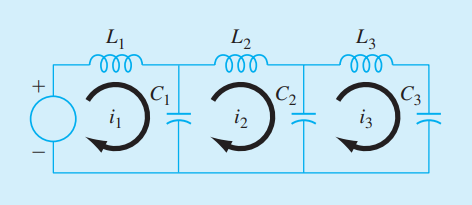
\includegraphics[width=0.75\textwidth]{fig_13_33}
	   \label{fig:fig_13_33}
\end{figure}

Use MATLAB's eig command to solve for the eigenvalues
of the $k - m\omega^{2}$ matrix above. Then use these eigenvalues to
solve for the frequencies ($\omega$). Let $m_{1} = m_{2} - m_{3} - 1 kg$ , and
$k = 2 N/m$.
13.6 As displayed in Fig. P13.6, an LC circuit can be modeled by the following system of differential equations

\begin{equation}
L_{1}\frac{d^{2}i_{1}}{dt^{2}}+\frac{1}{C_{1}}(i_{1}-i_{2})=0
\end{equation}

\begin{equation}
L_{2}\frac{d^{2}i_{2}}{dt^{2}}+\frac{1}{C_{2}}(i_{2}-i_{3})-\frac{1}{C_{1}}(i_{1}-i_{2})=0
\end{equation}

\begin{equation}
L_{3}\frac{d^{2}i_{3}}{dt^{2}}+\frac{1}{C_{3}}i_{3}-\frac{1}{C_{2}}(i_{2}-i_{3})=0
\end{equation}


where L = inductance (H), t = time (s), i = current (A), and
C = capacitance (F). Assuming that a solution is of the form
ij = Ij sin ($\omega$t), determine the eigenvalues and eigenvectors for
this system with L = 1 H and C = 0.25C. Draw the network,
illustrating how the currents oscillate in their primary modes.
13.7 Repeat Prob. 13.6 but with only two loops. That is,
omit the i3 loop. Draw the network, illustrating how the currents oscillate in their primary modes.
13.8 Repeat the problem in Sec. 13.5 but leave off the third
floor.
13.9 Repeat the problem in Sec. 13.5 but add a fourth floor
with m4 = 6,000 and k4 = 1,200 kN/m.

\begin{figure}[H]
		\centering
		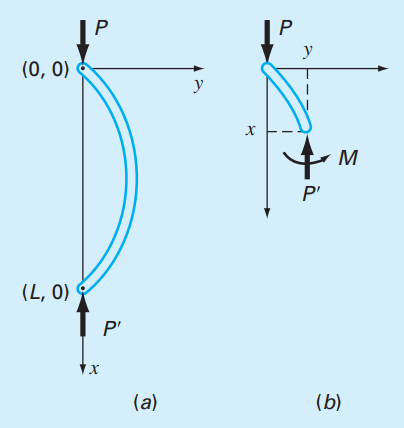
\includegraphics[width=0.75\textwidth]{fig_13_35}
	   \caption{\textsf{a) A slender rod. (b) A freebody diagram of a rod.}}
	   \label{fig:fig_13_35}
\end{figure}

13.10 The curvature of a slender column subject to an axial
load P (Fig. P13.10) can be modeled by

\begin{equation}
\frac{d^{2}y}{dx^{2}}+p^{2}y=0
\end{equation}

where
\begin{equation}
p^{2}=\frac{P}{EI}
\end{equation}

where E = the modulus of elasticity, and I = the moment of
inertia of the cross section about its neutral axis.
This model can be converted into an eigenvalue problem
by substituting a centered finite-difference approximation
for the second derivative to give

\begin{equation}
\frac{y_{i+1}-2y_{i}+y{i-1}}{\Delta x^{2}}+p^{2}y_{i}=0
\end{equation}

where i = a node located at a position along the rod's interior, and $\delta x=$ the spacing between nodes. This equation can
be expressed as
\begin{equation}
y_{i-1}-(2-\Delta x^{2}p^{2})y_{1}+y_{i+1}=0
\end{equation}

Writing this equation for a series of interior nodes along the
axis of the column yields a homogeneous system of equations. For example, if the column is divided into five segments (i.e., four interior nodes), the result is
\begin{equation}
\begin{bmatrix}
(2-\Delta x^{2}p^{2}) & -1 & 0 &0 \\
 & (2-\Delta x^{2}p^{2}) &  & \\
 0& -1 &-1 (2-\Delta x^{2}p^{2}) & 0\\
 0& 0 & -1 & (2-\Delta x^{2}p^{2})
\end{bmatrix}
\end{equation}

n axially loaded wooden column has the following characteristics: $E = 10 × 10^{9} Pa$, $I = 1.25 × 10^{-5} m^{4}$, and L = 3 m.
For the five-segment, four-node representation:

\begin{enumerate}[label=\alph*]
\item Implement the polynomial method with MATLAB to
determine the eigenvalues for this system.
\item Use the MATLAB eig function to determine the eigenvalues and eigenvectors.
\item Use the power method to determine the largest eigenvalue and its corresponding eigenvector
\end{enumerate}

13.11 A system of two homogeneous linear ordinary differential equations with constant coefficients can be written as
\begin{equation}
\frac{dy_{1}}{dt}=-5y_{1}+3y_{1}
y_{1}(0)=50
\end{equation}

\begin{equation}
\frac{dy_{y}}{dt}=100y_{1}-301y_{2}
y_{2}(0)=100
\end{equation}

If you have taken a course in differential equations, you
know that the solutions for such equations have the form
\begin{equation}
y_{i}ce^{\lambda t}
\end{equation}

where c and $\lambda$ are constants to be determined. Substituting
this solution and its derivative into the original equations
converts the system into an eigenvalue problem. The resulting eigenvalues and eigenvectors can then be used to derive
the general solution to the differential equations. For example, for the two-equation case, the general solution can be
written in terms of vectors as

\begin{equation}
\{y\}=c_{1}\{v_{1}\}e^{\lambda_{1}t}+c_{2}\{v_{2}\}e^{\lambda_{2}t}
\end{equation}

where $\{v_{i}\}$ = the eigenvector corresponding to the i
th eigenvalue ($\lambda_{1}$) and the c's are unknown coefficients that can be
determined with the initial conditions.

\begin{enumerate}[label=\alph*]
\item Convert the system into an eigenvalue problem.
\item se MATLAB to solve for the eigenvalues and eigenvectors.
\item Employ the results of (b) and the initial conditions to
determine the general solution.
\item Develop a MATLAB plot of the solution for t = 0 to 1.
\end{enumerate}

13.12 Water flows between the North American Great
Lakes as depicted in Fig. P13.12. Based on mass balances,
the following differential equations can be written for the
concentrations in each of the lakes for a pollutant that decays
with first-order kinetics:

\begin{figure}[H]
		\centering
		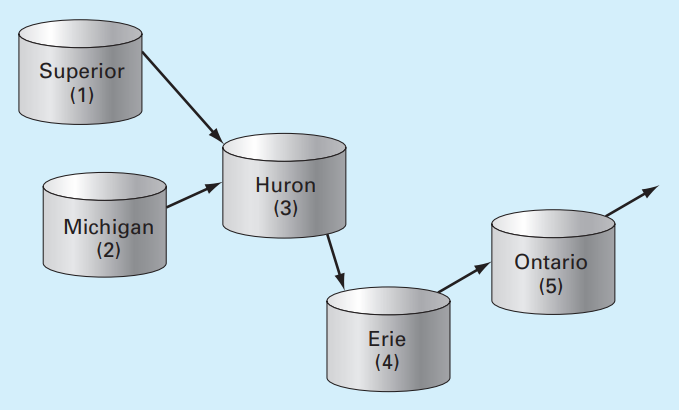
\includegraphics[width=0.75\textwidth]{fig_13_36}
	   \caption{\textsf{a) The North American Great Lakes. The arrows indicate how water
flows between the lakes.}}
	   \label{fig:fig_13_36}
\end{figure}

\begin{equation}
\frac{dc_{1}}{dt}=-(0.0056+k)c_{1}
\end{equation}

\begin{equation}
\frac{dc_{2}}{dt}=-(0.01+k)c_{2}
\end{equation}

\begin{equation}
\frac{dc_{3}}{dt}=0.01902c_{1}+0.01387c_{2}-(0.047+k)c_{3}
\end{equation}

\begin{equation}
\frac{dc_{4}}{dt}=0.33597c_{3}-(0.376+k)c_{4}
\end{equation}

\begin{equation}
\frac{dc_{5}}{dt}=0.11364c_{4}-(0.133+k)c_{5}
\end{equation}
where k = the first-order decay rate (/yr), which is equal to
0.69315/(half-life). Note that the constants in each of the equations account for the flow between the lakes. Due to the
testing of nuclear weapons in the atmosphere, the concentrations of strontium-90 $(^{90}Sr)$ in the five lakes in 1963 were
approximately $\{c\} = \{17.7 30.5 43.9 136.3 30.1\}^{T}$ in units
of $Bq/m^{3}$
. Assuming that no additional $(^{90}Sr)$ entered the system thereafter, use MATLAB and the approach outlined in
Prob. 13.11 to compute the concentrations in each of the
lakes from 1963 through 2010. Note that $(^{90}Sr)$ has a half-life
of 28.8 years.
13.13 Develop an M-file function to determine the largest
eigenvalue and its associated eigenvector with the power
method. Test the program by duplicating Example 13.3 and
then use it to solve Prob. 13.2.

\end{document}
